\documentclass[9pt]{article}
\usepackage[utf8]{inputenc}
\usepackage{amsmath,amsthm,amsfonts,amssymb,amscd}
\usepackage{multirow,booktabs}
\usepackage{enumitem}
\usepackage{fancyhdr}
\usepackage{mathrsfs}
\usepackage{wrapfig}
\usepackage{setspace}
\usepackage{calc}
\usepackage{multicol}
\usepackage{cancel}
\usepackage[retainorgcmds]{IEEEtrantools}
\usepackage{framed}
\usepackage[most]{tcolorbox}
\usepackage{tikz}
\usepackage{geometry}
\geometry{
	a4paper,
	total={170mm,257mm},
	left=20mm,
	top=20mm,
}
\title{Magnetic Fields \& Forces}
\author{Aaron G.K.}
\begin{document}
	\maketitle
	\begin{center}
	\section*{Magnetic Fields}
	\end{center}	
	\subsection*{Force Fields}
	Early on in dynamics, we have seen that we can categorize forces as being \textbf{contact} or \textbf{non-contact} based on the need of contact in order for the force to be experienced. Non-contact forces act over distance and their pattern of action is determined by a \textbf{force field} - a region in which the non-contact force is exerted and felt.\\ \\
	Common examples of non-contact forces include gravitation, magnetic force, and electric force. One thing common about them all? They all act over space(\textit{action at a distance}) and don't necessarily need contact in order to be felt. 
	\subsection*{Magnetic Fields}
	Magnetic Fields are no different from other non-contact forces in that they act over a distance. We have seen in Electrostatics that the \textit{Coulomb	Force} acts on the electric field. Electric Field is projected radially outwards from a positive charge and radially inwards in a negative charge. The source of any magnetic field possesses two poles, a \textbf{north pole} and a \textbf{south pole}. The poles received their names because of the way a magnet, such as that in a compass, behaves in the presence of the Earth’s magnetic field when suspended freely. \\ 
	As with positive charges, magnetic field lines come out of the north pole. Similar to negative charges, magnetic field lines go inside the south pole of a magnet. If we draw the magnetic field lines across a bar magnet, we can see the following pattern. \\
	\begin{center}
	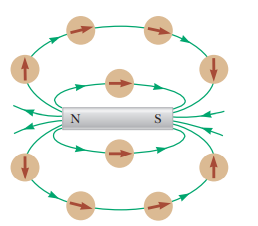
\includegraphics[scale=0.5]{magnetic_field_bar.png}	
	\end{center}
	The magnetic field lines outside a magnet start from the North Pole and go into the South, while inside the magnet it goes from the South to the North pole. It is a universal characteristic of all magnets that like poles repel and unlike poles attract, however, it is impossible to separate a magnetic pole on its own. \\ \\
	\section*{Magnetic Field, Force and Sources}
	We have said earlier that magnetic force is a non-contact force and that it acts over a field. To visualize a magnetic field, we use hypothetical field lines that show how the magnetic force acts over the space. Here is an example of a magnetic field acting on iron fillings. \\
	\begin{center}
	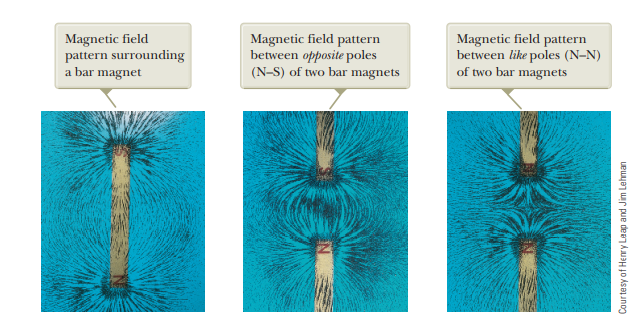
\includegraphics[scale=0.5]{magnetic_field_patterns.png}	
	\end{center}
	There are multiple sources of magnetic field. A straight current carrying wire is one prime example of a source of magnetic field. The magnetic field generated by a straight current carrying wire is determined by the \textbf{Right Hand Rule}. The basic idea in this rule is to align your thumb with the direction of current(\textbf{I}). Then, the direction in which the rest of your fingers curl show the direction of the magnetic field(\textbf{B}).
	\subsection*{Magnetic Force on Moving Charges}
	We have seen in the introduction of magnetism that charges respond to electromagnetic fields. Thus, we can infer that charges will be acted up on by a force when present in a magnetic field.	To define magnetic field, however, we have to define the magnetic force first. That is because, unlike electrical charges, magnetic poles don't have monopoles and the only way we can define the field is through the magnetic force. To achieve that experiments have been done and we tested the magnetic force on moving charges to find out the following:
	\begin{itemize}
		\item Magnetic force exists only when the charge is in motion relative to the magnetic field.
		\item Not only should the charge be in motion, its velocity should have a perpendicular component to the magnetic field. (No force exists when the charge is moving parallel to the magnetic field)
		\item The magnetic force exerted is perpendicular to the direction of the magnetic field( unlike the electrostatic force which is in the same direction) and it is also perpendicular to the velocity of the charge. Hence, no work is done by the magnetic force.
		\item The magnetic force is directly proportional to the magnitudes of the charge, velocity \& magnetic field.
	\end{itemize}
	As we saw properties of vectors in the previous lesson, it is easy to summarize the above observations using a single equation and that equation makes use of the vector product.
	$$\vec{F}=q\vec{v}\times\vec{B}$$	
	From the above vector product we see that $\vec{F}$ is perpendicular to the plane containing $\vec{B}$ and $\vec{V}$. Since it is a vector product, we can also see that the maximum value is attained when $\vec{V}$ and $\vec{B}$ are perpendicular but minimum(zero) when the two are parallel. \\ \\
	To calculate the magnitude of the force, we can use the method we used in vector products as follows: 
	$$F=qvB\sin\theta$$
	From this expression, we can define the magnetic field now that we have formally defined the magnetic force. As such, the magnetic field is given as follows:
	$$B=\dfrac{F}{qv\sin\theta}$$
	The magnetic field strength has an SI unit of Tesla(\textit{after Nikola Tesla}) and we can express Tesla in terms of the other SI units.
	$$1 \text{T}=\dfrac{N}{\text{C}\times\text{m/s}}=1\dfrac{N}{Am}$$
	Since Tesla is a large unit of magnetic field to find within our close proximity, we use smaller quantities of magnetic field such as the Gauss when dealing with quantities that are common, which is ten thousandth of a Tesla. $1 G = 10^{-4}$T.
	\subsection*{Motion of Charged Bodies in Uniform Magnetic Fields}
	 We have seen from the property of cross product above that the magnetic force is always perpendicular to velocity, so that it does no work on the charged particle. That means, the particle’s kinetic energy and speed remain constant. The direction of motion is affected and changes every instant, but not the speed. This is typical of uniform circular motion and the simplest case occurs when a charged particle moves perpendicular to a uniform  magnetic field. \\ \\
	 For an object moving about a circular trajectory, the net force on the object is the centripetal force. For a charged particle exclusively in a magnetic field, the only force acting on it is the magnetic force. Thus the net force on the charged particle (and hence, the centripetal force) is equal to the magnetic force. Mathematically, we can express it as shown below by relating the radius of the trajectory of the charged particle with its mass and the magnetic field it is in.
	 $$F_{net}=F_{magnetic}\implies F_{c}=F_{magnetic}$$
	 $$\dfrac{mv^2}{r}=qvB\sin\theta$$
	 $$r=\dfrac{mv}{qB\sin\theta}$$	 
	 \begin{center}
	 	\includegraphics*[scale=0.3]{charged_circular_path.jpg}
	 \end{center}
 	 This concept has important applications in real life including its use in mass spectrometry in which magnetic fields are used to measure the masses of various particles that enter the spectrometer. Not only is this concept useful in real life, but also we can usually observe this phenomenon in real life including the Aurora Borealis.  Charged particles approaching magnetic field lines may get trapped in spiral orbits about the lines rather than crossing them, as seen above. Some cosmic rays, for example, follow the Earth’s magnetic field lines, entering the atmosphere near the magnetic poles and causing the southern or northern lights through their ionization of molecules in the atmosphere. Those particles that approach middle latitudes must cross magnetic field lines, and many are prevented from penetrating the atmosphere. Cosmic rays are a component of background radiation; consequently, they give a higher radiation dose at the poles than at the equator.
 	 \subsection*{Magnetic Force on a Current-Carrying Conductor}
 	 We have seen that force is exerted on moving charges in an electric field, so it is only fair to assume that there will be force exerted when there's multiple of them, i.e., when current is present. Thus, if there is a current carrying wire present in an external magnetic field, magnetic force might be exerted on it. Let's try to express it using a simple mathematical model. \\ \\
 	 We can take the force on the current carrying wire as the total force acting on each charge in the wire, but instead of taking the individual velocities of each charge, we use the drift speed.
 	 $$F = \left(qv_{d}B \sin \theta \right) \left(N\right)$$
 	 But, we have seen from the idea of current and drift speed that $N=nV$ such that n is electron density while the volume can be expressed as the product of the cross-sectional area and length of the conducting wire - $V=Al$.
 	 $$F = \left(qv_{d}B \sin \theta \right) \left(nV\right)$$
 	 $$F = \left(qv_{d}B \sin \theta \right) \left(nAl\right)$$
 	 $$F = \left(nqAv_{d}\right)lB\sin\theta$$
 	 But, we know that $I=nqAv_{d}$, thus:
 	 $$F = IlB\sin\theta$$
 	 Another simpler way to think of this is to start of the the force on a moving charge and build up on it:
 	 $$\vec{F}=q\vec{V}\times\vec{B}$$
 	 $$\vec{F}=q\dfrac{\vec{S}}{t}\times\vec{B}$$
 	 $$\vec{F}=\dfrac{q}{t}\vec{S}\times\vec{B}$$
 	 $$\vec{F}=I\vec{S}\times\vec{B}$$
 	 However, $\vec{S}$ is the distance the charges travel which is the total length of the conductor. Since the length itself is not a vector, we define it to be a vector that has a magnitude equal to the length of the conductor and a direction the same as the conventional current.
 	 $$\vec{F}=I\vec{l}\times\vec{B}$$
 	 \subsection*{Magnetic Fields Produced by Currents}
 	 The first time we ever scientifically linked electricity with magnetism is when Oersted discovered in 1820 that a current in a wire affected a compass needle, he was not dealing with extremely large currents. This is remarkable because the two seemingly unrelated phenomena of electricity and magnetism were found to be related -in fact they birth one another. \\ \\
	 The magnetic field of current carrying wires mainly depends on the amount of current being carried in the wires and the geometry of the wires. The simplest of these situations such as the one observed by Oersted is manifested in a straight current carrying wire. For straight current carrying wires, the magnetic field is given by:
	 $$B=\dfrac{\mu_0I}{2\pi a}\text{, such that a is the radial distance from the wire.}$$
	 $\mu_0$ is a constant called the permeability of free space or it is generally called the \textbf{magnetic constant}. \\
	 As magnetic field is a vector quantity, we also need a direction to indicate where the field is acted. To do that we use a Right Hand Rule in such a way that the thumb of our right hand points to the direction of the conventional current while the rest of the fingers indicate the direction of the field. 
	 \begin{center}
	 	\includegraphics*[scale=0.6]{rhr.jpg}
	 \end{center}
	 We can also see that the magnetic fields induced by straight current carrying are always circular. \\ \\
	 For other geometrical structures of wires such as current carrying loops, we use Ampere's Law to calculate the magnetic fields induced by them.
	 \subsection*{Force Between Current Carrying Wires}
	 In the above sections, we have seen two important things: 
	 \begin{itemize}
	 	\item When a current carrying wire is inserted into an external magnetic field, magnetic force is exerted by the field on the wire.
	 	\item A current carrying wire can produce a magnetic field of its own.
	 \end{itemize}
 	 From the above two statements we can definitely infer that there is an interaction between two current carrying wires because when one of the wires acts as a source of the magnetic field, the other one will experience magnetic force exerted on it. \\
 	 \begin{center}
 	 	\includegraphics*[scale=0.7]{two_wires.jpg}
 	 \end{center}
  	 For example, we can look at the wire 1 and calculate the force it exerts on wire 2. To do that, we first need to calculate the magnetic field on wire 2 due to wire 1.
  	 $$B_1=\dfrac{\mu_0I_1}{2\pi r}$$
  	 However, when calculating for the force on wire 2, I need to use the current passing through wire 2 and its length as I would normally 2. Thus,
  	 $$F_{12}=I_2L_2B_1$$
  	 $$F_{12}=I_2L_2\dfrac{\mu_0I_1}{2\pi r}$$
  	 We can find the direction of the forces using the right hand rule or the vector products. \\ \\
  	 The direction of $\vec{l}_2$ is upwards ($\hat{j}$) while that of $\vec{B}_1$ is into the page ($-\hat{k}$)  
  	 $$\vec{F}_{12}=I_2\vec{l}_2\times\vec{B}_1$$
  	 $$\vec{F}_{12}=\hat{j}\times-\hat{k}$$
  	 $$\vec{F}_{12}=-\hat{i}$$
  	 This indicates that wire 2 will be pulled to the left by wire 1. \\ \\
  	 For the force exerted by wire 2 on wire 1, we have the exact opposite: the magnetic field is due to wire 2, but we use the length of and current in wire 1 since we are calculating the force on wire 1. In that case, we have the following:
  	 $$B_2=\dfrac{\mu_0I_2}{2\pi r}$$
  	 $$F_{21}=I_1L_1B_2$$
  	 $$F_{21}=I_1L_1\dfrac{\mu_0I_2}{2\pi r}$$
  	 Similarly to the steps above, we can find the direction of the forces using the right hand rule or the vector products. \\ \\
  	 The direction of $\vec{l}_1$ is upwards ($\hat{j}$) while that of $\vec{B}_2$ is out of the page ($\hat{k}$)  
  	 $$\vec{F}_{21}=I_1\vec{l}_1\times\vec{B}_2$$
  	 $$\vec{F}_{21}=\hat{j}\times\hat{k}$$
  	 $$\vec{F}_{21}=\hat{i}$$
  	 This indicates that wire 1 will be pulled to the right by wire 2. This means that the wires 1 and 2 attract one another. Generally, if a current is flowing in the same direction in two current carrying wires, the wires attract. \\ \\
  	 \textbf{TO DO}: Show that current carrying wires repel when the current is flowing in opposite directions in the two wires.
  	 
\end{document}	